\section{Correlation Calculation}
\label{sec:calculation}
\subsection{Global Index}
\label{subsec:global-index}

We use a global index to record all the distance information. Each vertex of the data graph stores two catogories of distance information.

\squishlist
\item{\bf Proximity Vertices.} For each $u\in G$, we store the information of proximity vertices of $u$, denoted as $CorV(u)$, for each vertex $u\in CorV(u)$, there exists $d(u,v)\le h$.
\squishend
\squishlist
\item{\bf Proximity Patterns.} For each $u\in G$, we store the information of proximity patterns of $u$, denoted as $CorP(u)$, for each pattern $Q\in CorP(u)$, suppose the instance-groups of $Q$ is $\mathbb{I'}=\{I'_1,I'_2,\ldots,I'_{\sigma(Q)}\}$, there exists $I'\in \mathbb{I'}$, $\exists v\in I'$, $d(u,v)\le h$.
\squishend
With the global index acquired before the search, there is no need to consider anything about the distance (hop-constraints) in the search steps. The detail of the maintenance of these two indices is specified in Section \ref{subsec:calculating}.

\subsection{Calculating Correlation}\label{subsec:calculating}
\begin{defn}[Positive Instance Group]
Given two subgraphs $Q_1$ and $Q_2$ in the input graph $G$, their instance-groups
$\mathbb{I'}=\{I'_1,I'_2,\ldots,I'_{\sigma(Q_1)}\}$ and $\mathbb{J'}=\{J'_1,J'_2,\ldots,J'_{\sigma(Q_2)}\}$,
respectively, and a user-defined distance-threshold $h$, assume that $\sigma(Q_1) \le \sigma(Q_2)$. 
Then, we say an instance group of $Q_1$, $I'_i\in \mathbb{I'}$ is a {\bf positive instance group} of $Q_2$ if following condition is satisfied.
%
\begin{align}
\exists J' \in \mathbb{J}, \exists u \in I', \exists v \in J', d(u,v)\le h
\end{align}
Then, we denote $P(I'_i,Q_2,h)=1$, otherwise $P(I'_i,Q_2,h)=0$.
\end{defn}	
\begin{thrm}
	Let $Q_1,Q_2$ be two subgrpah patterns, and an instance group of $Q_1$, $I'$. Then,	if $Q_2\in \cap CorP(v),v\in I'$, $P(I'_i,Q_2,h)=1$.
	otherwise, $P(I'_i,Q_2,h)=0$.
\end{thrm}	
The process of correlation calculation could be considered as a {\bf collection}. Suppose we are calculating the correlation of $Q_1$, i.e. $\tau(Q_1,Q_k,h)$, for all $Q_k\in Cor(T)$. Taking advantage of the global index in Section \ref{subsec:global-index}, by traversing all the vertices in a group can we know the correlation $\tau()$ of all the $v$. We collect these sets one-by-one and finally we could know all the correlation of $Q_1$, i.e. $\tau(Q_1,Q_k,h)$, for all $Q_k\in Cor(T)$.

\subsubsection{Tree Structure Transformation}
It is more convenient to implement an efficient collection in a hierarchical structure, like tree. As a result, to initialize a collection, we first transform the search space of the collection to a particular tree.
\par Prior to the detailed operations, we first define the group center and the collection tree of a pattern.
\begin{defn}[Group Center and Center Subscript]
	Given a subgraph $Q$, and the instance-groups of $Q$, $\mathbb{I'}=\{I'_1,I'_2,\ldots,I'_{\sigma(Q)}\}$, a group center $u$ of $I'_i$ is the vertex having the minimum MNI support among all $v\in I'_i$, denoted as $u=center(I_i)$, a center subscript is the vertex subscript has the MNI support of the images, denoted as $centerSubscript(Q)$. i.e. $centerSubscript(Q)=i$, where $M(s_i)=\sigma(Q)$.
\end{defn}
\begin{defn}[Collection Tree]
	Given a subgraph $Q$, a collection tree of $Q$, $CT(Q)$ is tree transfromed from the tree structure replica, and rooted at $centerSubscript(Q)$.
\end{defn}
% First of all, if a subgraph contains any backward edges, we remove all its backward edges in its replica prior to the calculation. This is because 1) removing backward edges would not affect the result of correlation calculation. 2) removing backward edges could derive a tree structure subgraph, which is more convenient to carry out the collection.
\begin{figure}[t!]
\vspace{-2mm}
\centering
\subfigure[{\scriptsize Subgraph Pattern $Q_1$}] {
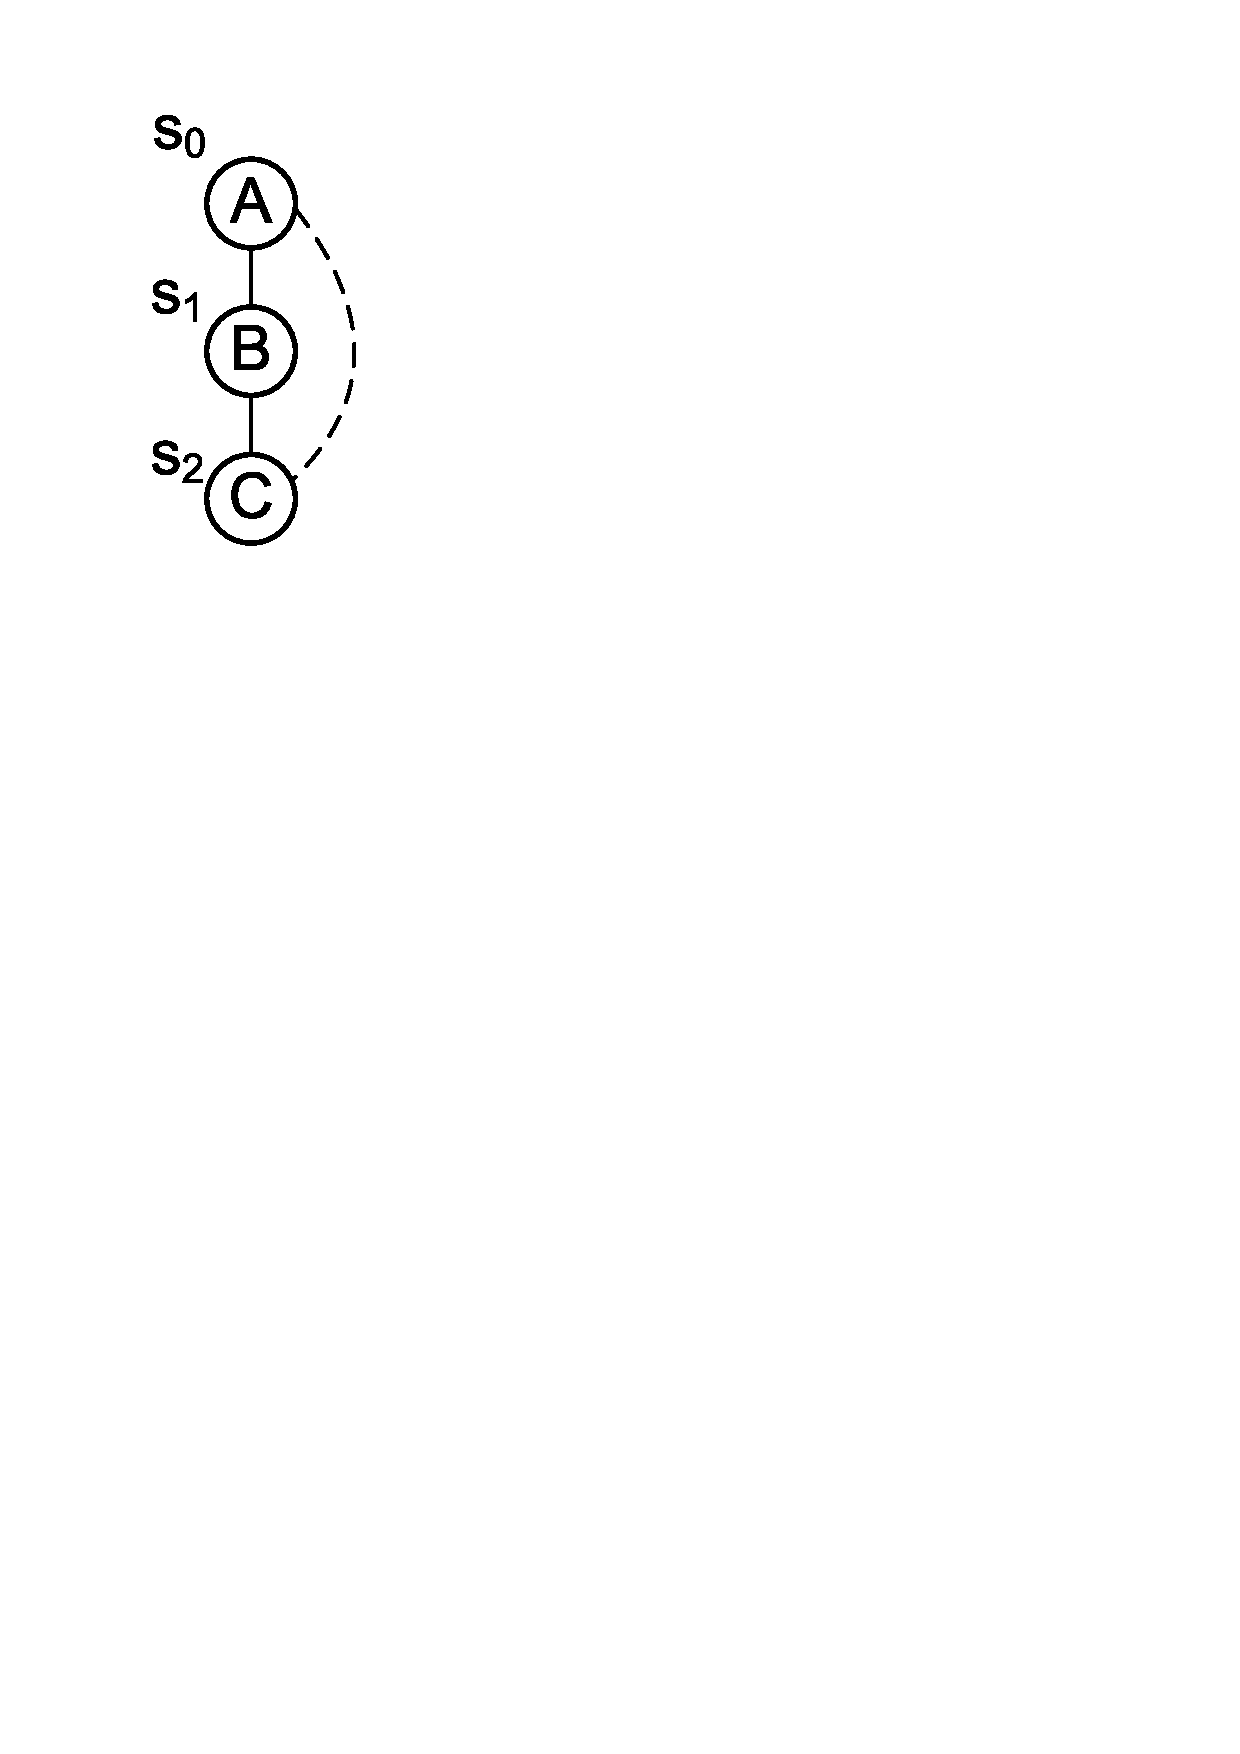
\includegraphics[scale=0.35]{images/tree_structure0}
\label{fig:tree_structure0}
}
\subfigure[{\scriptsize Occurrence of $Q_1$}] {
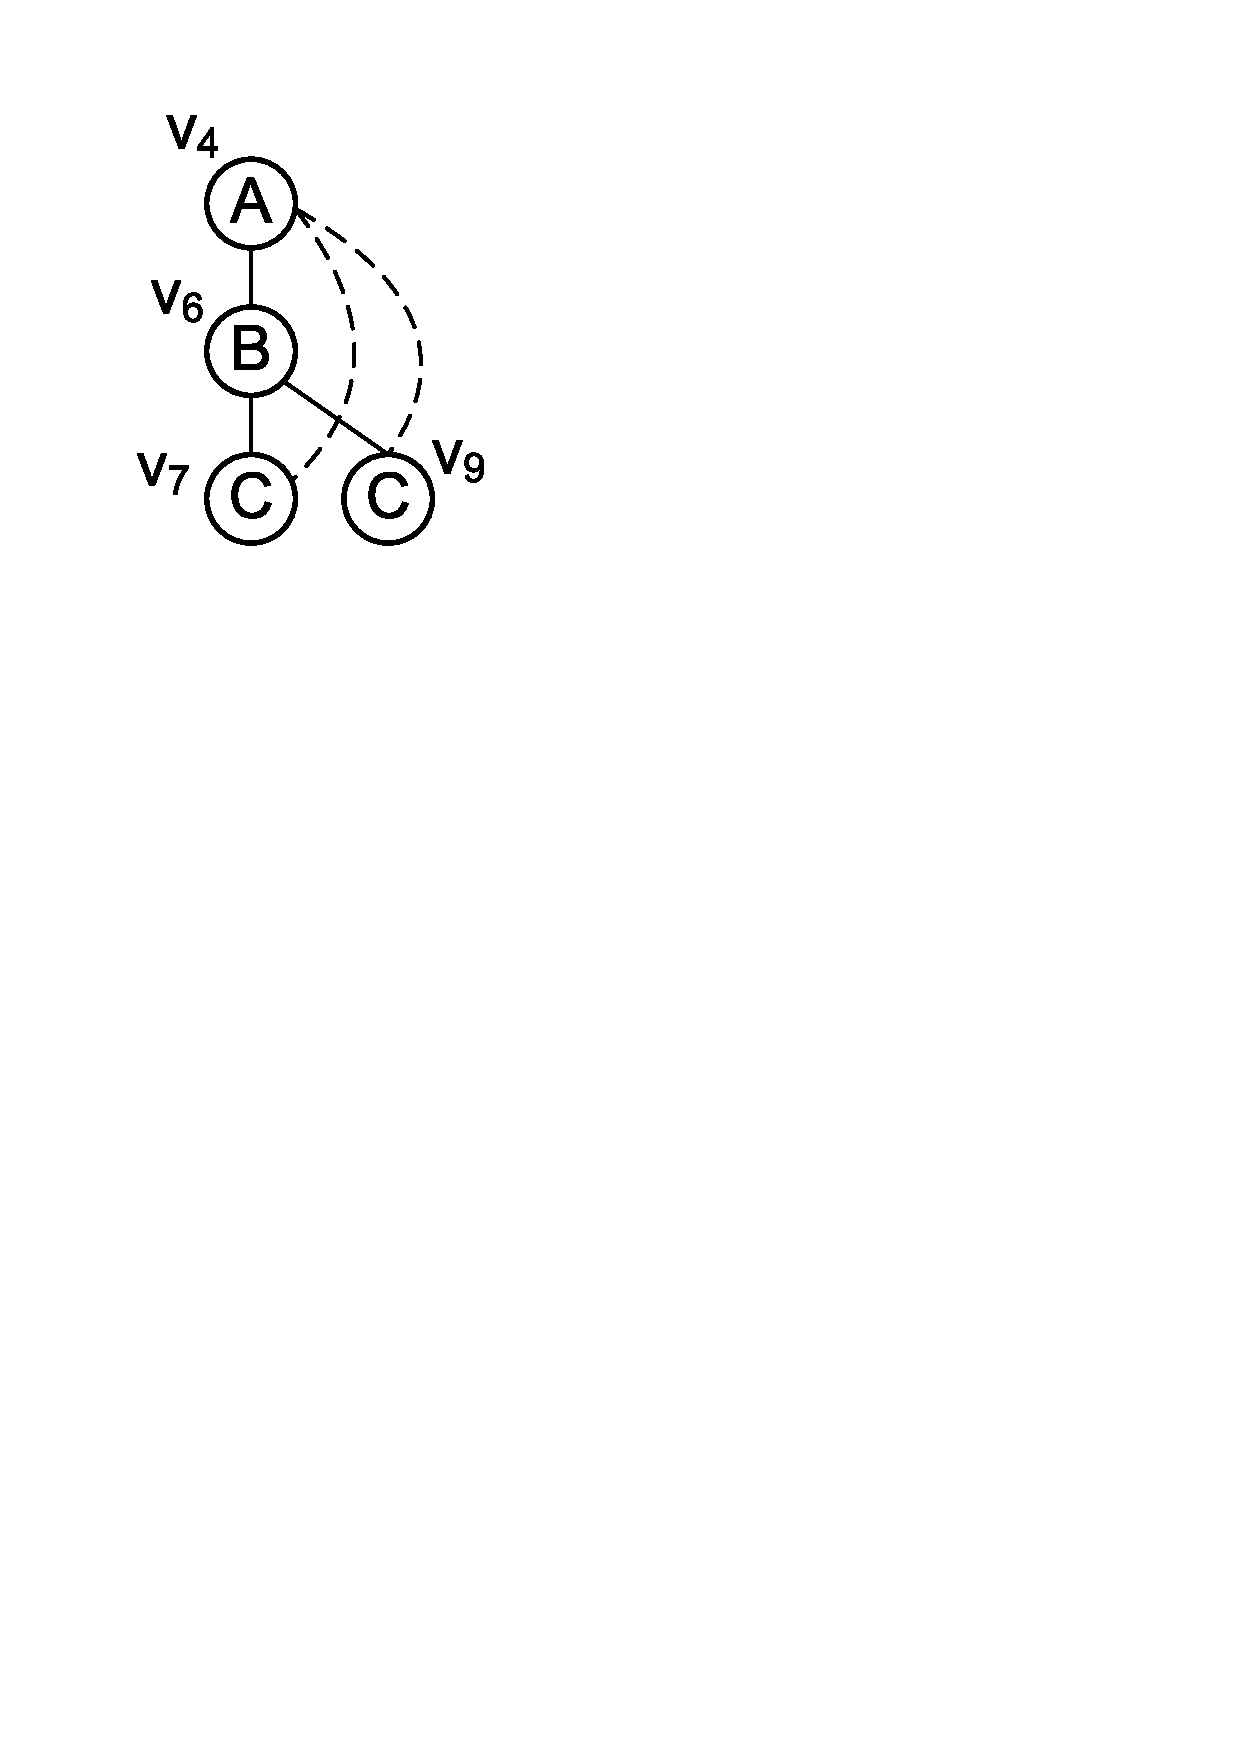
\includegraphics[scale=0.35]{images/tree_structure1}
\label{fig:tree_structure1}
}
\subfigure[{\scriptsize Replica of $Q_1$}]  {
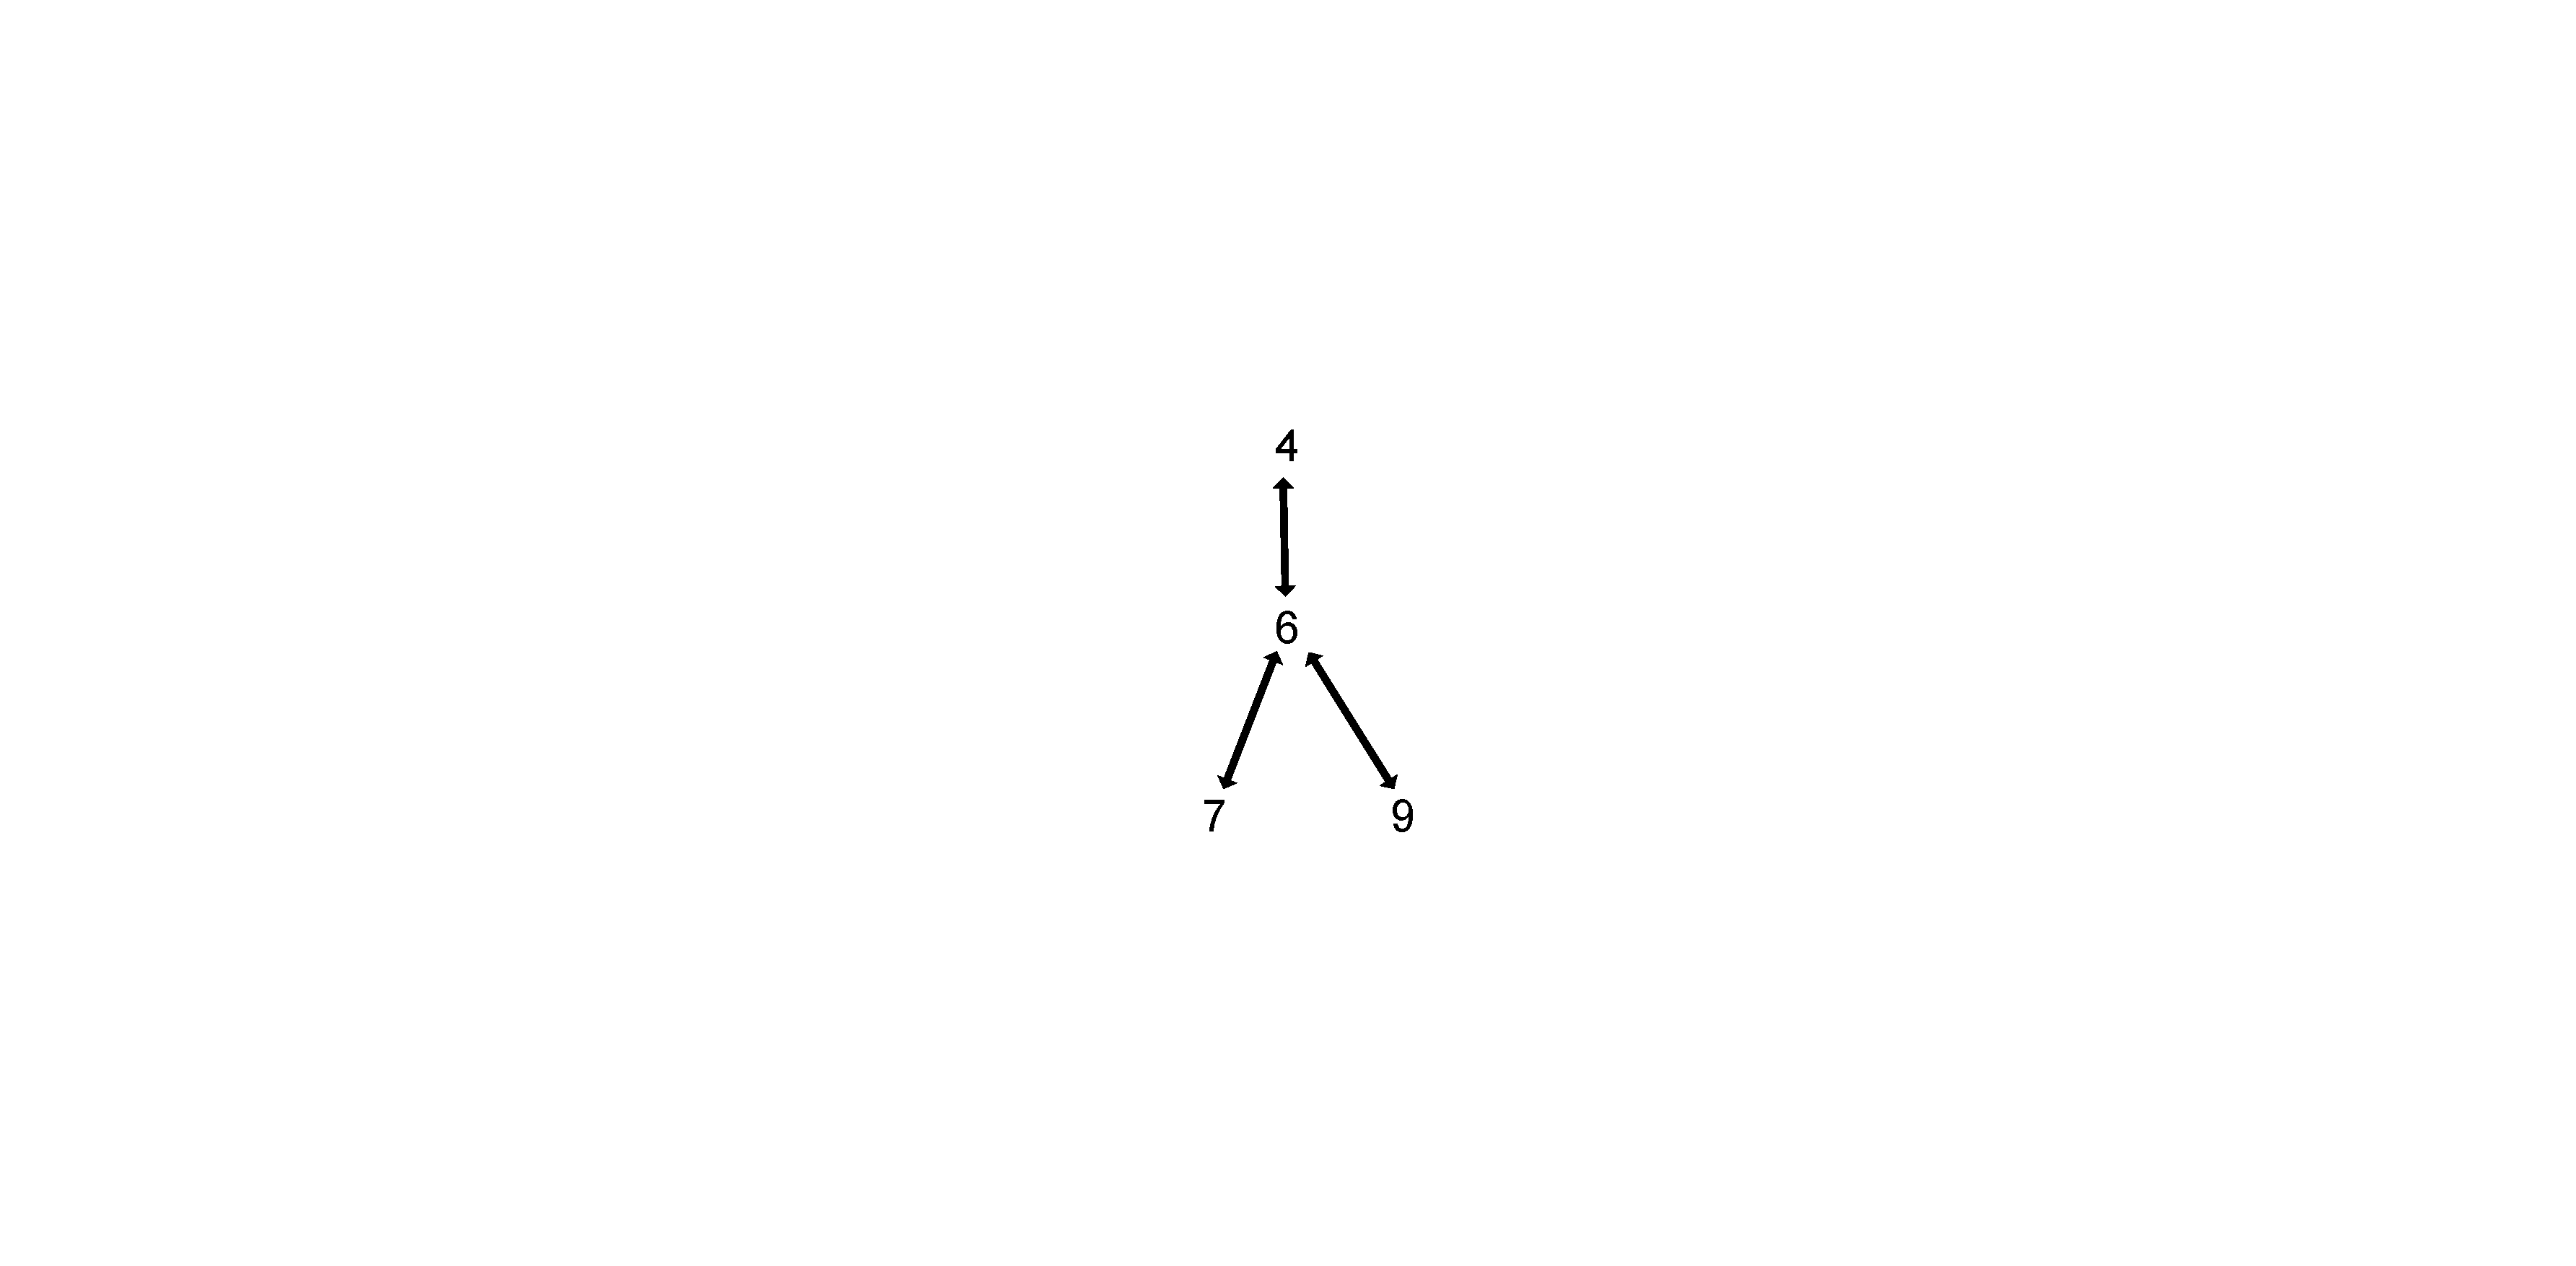
\includegraphics[scale=0.26]{images/tree_structure2}
\label{fig:tree_structure2}
}
\subfigure[{\scriptsize Subgraph Pattern $Q_2$}]  {
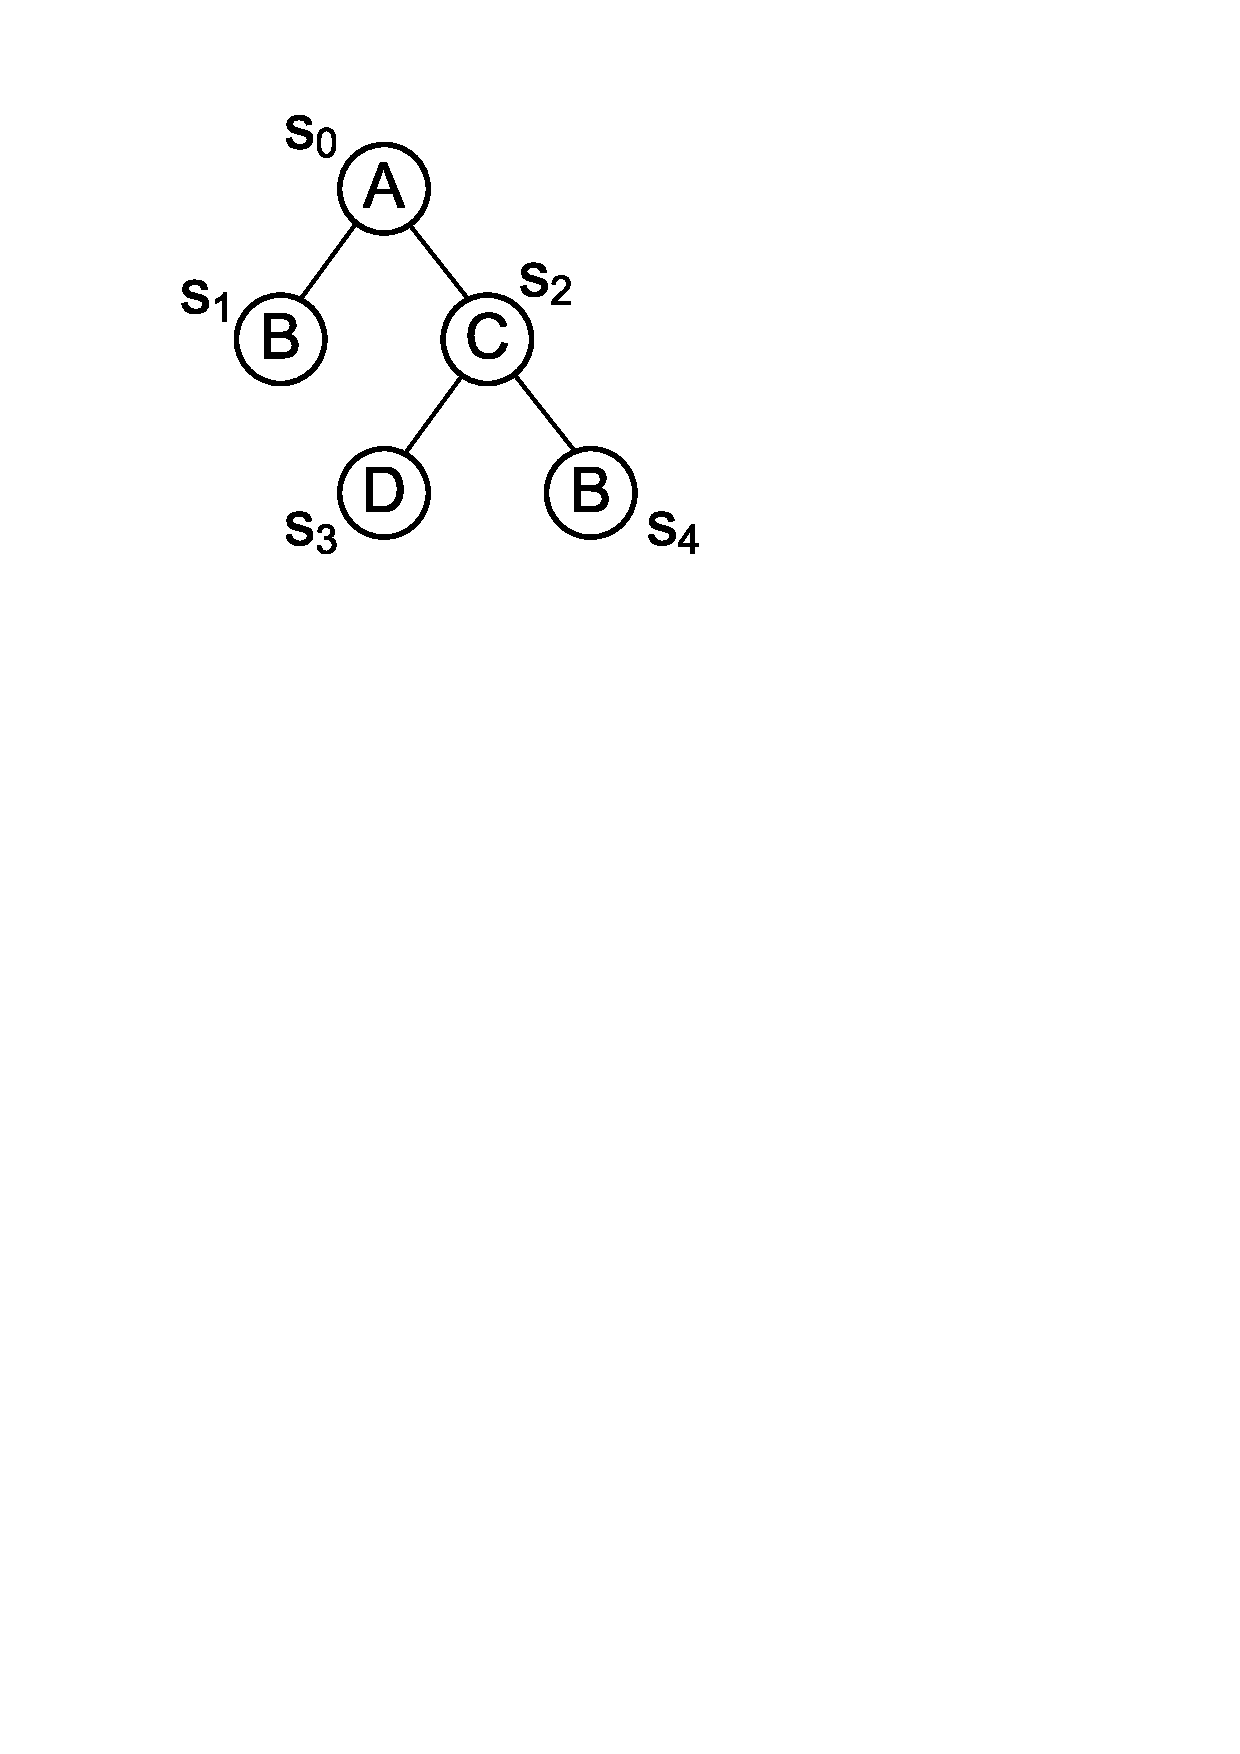
\includegraphics[scale=0.33]{images/tree_structure3}
\label{fig:tree_structure3}
}
\subfigure[{\scriptsize Collection Tree of $Q_2$}] {
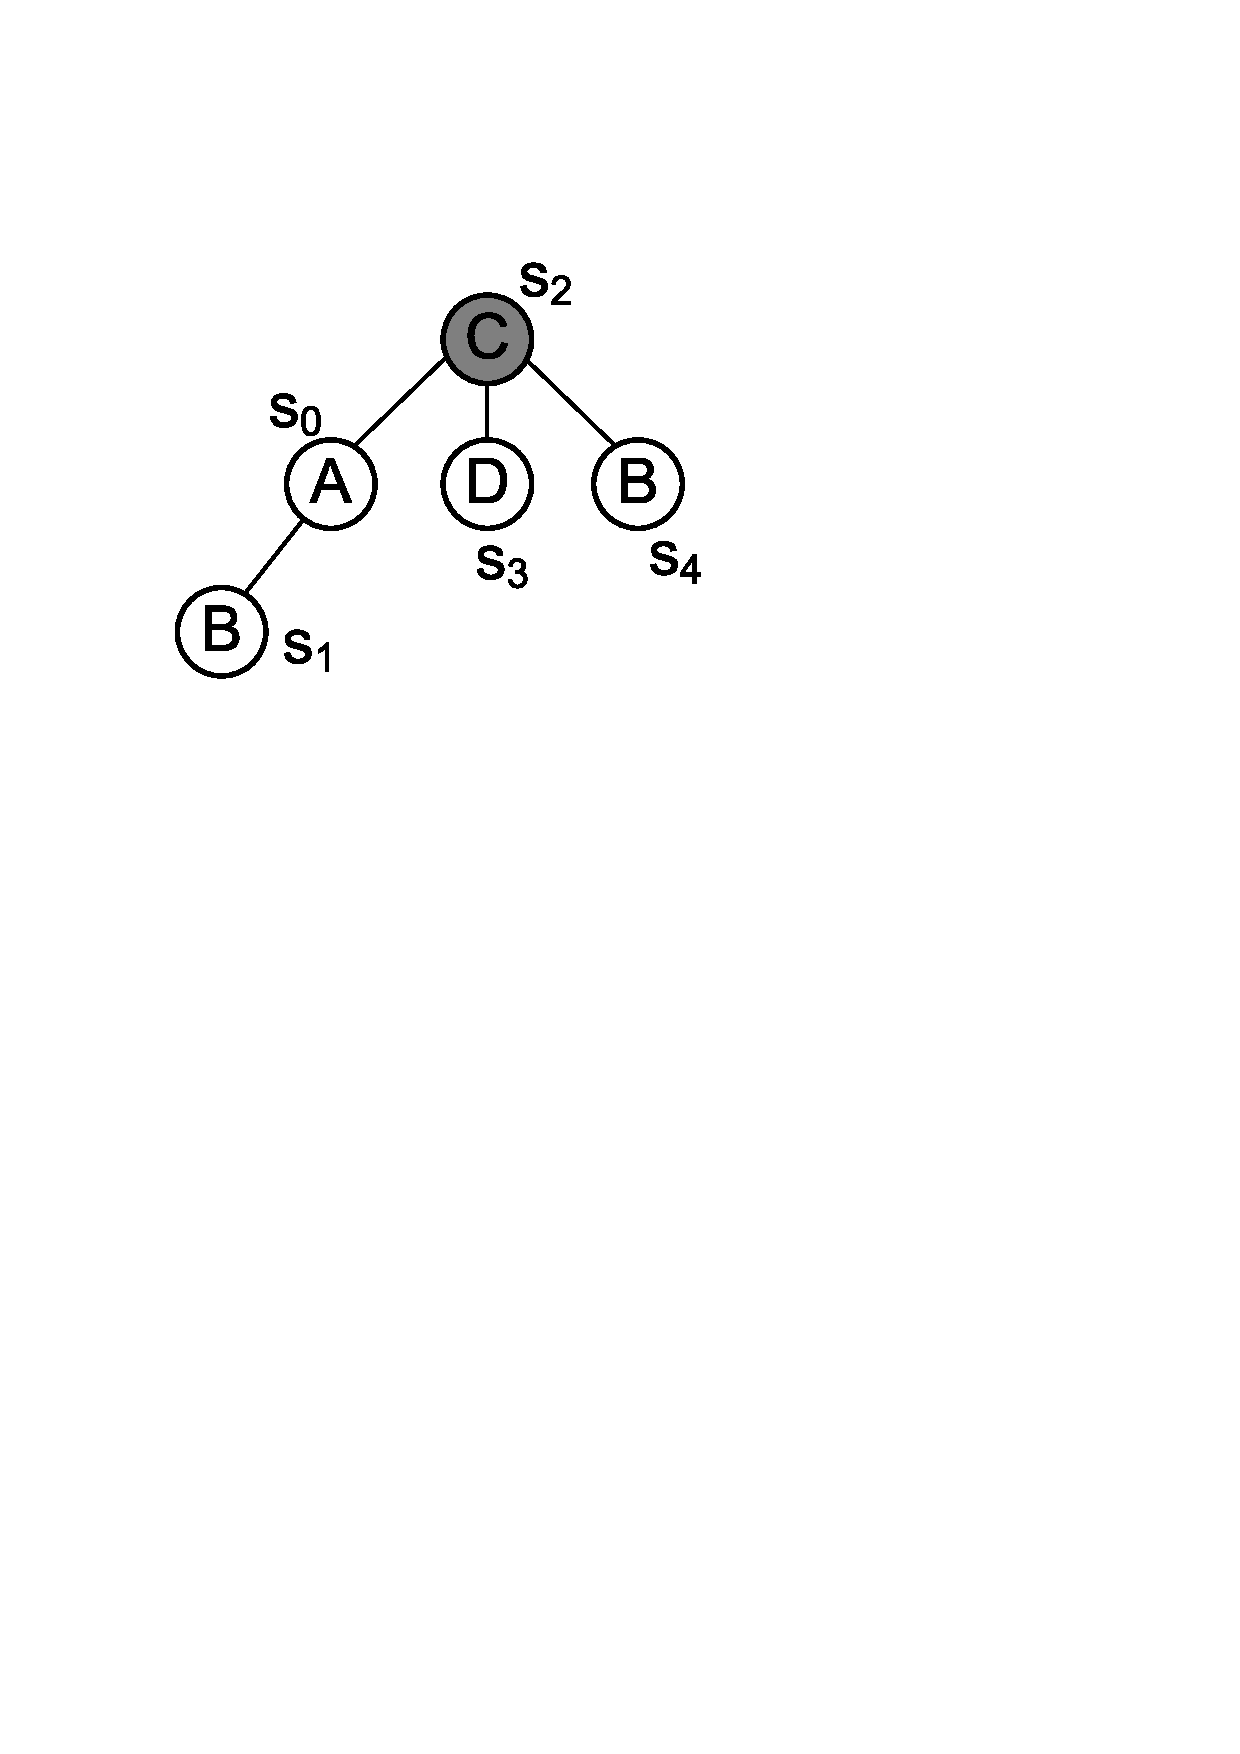
\includegraphics[scale=0.33]{images/tree_structure4}
\label{fig:tree_structure4}
}
\subfigure[{\scriptsize Occurrence of $Q_2$ in $G$}] {
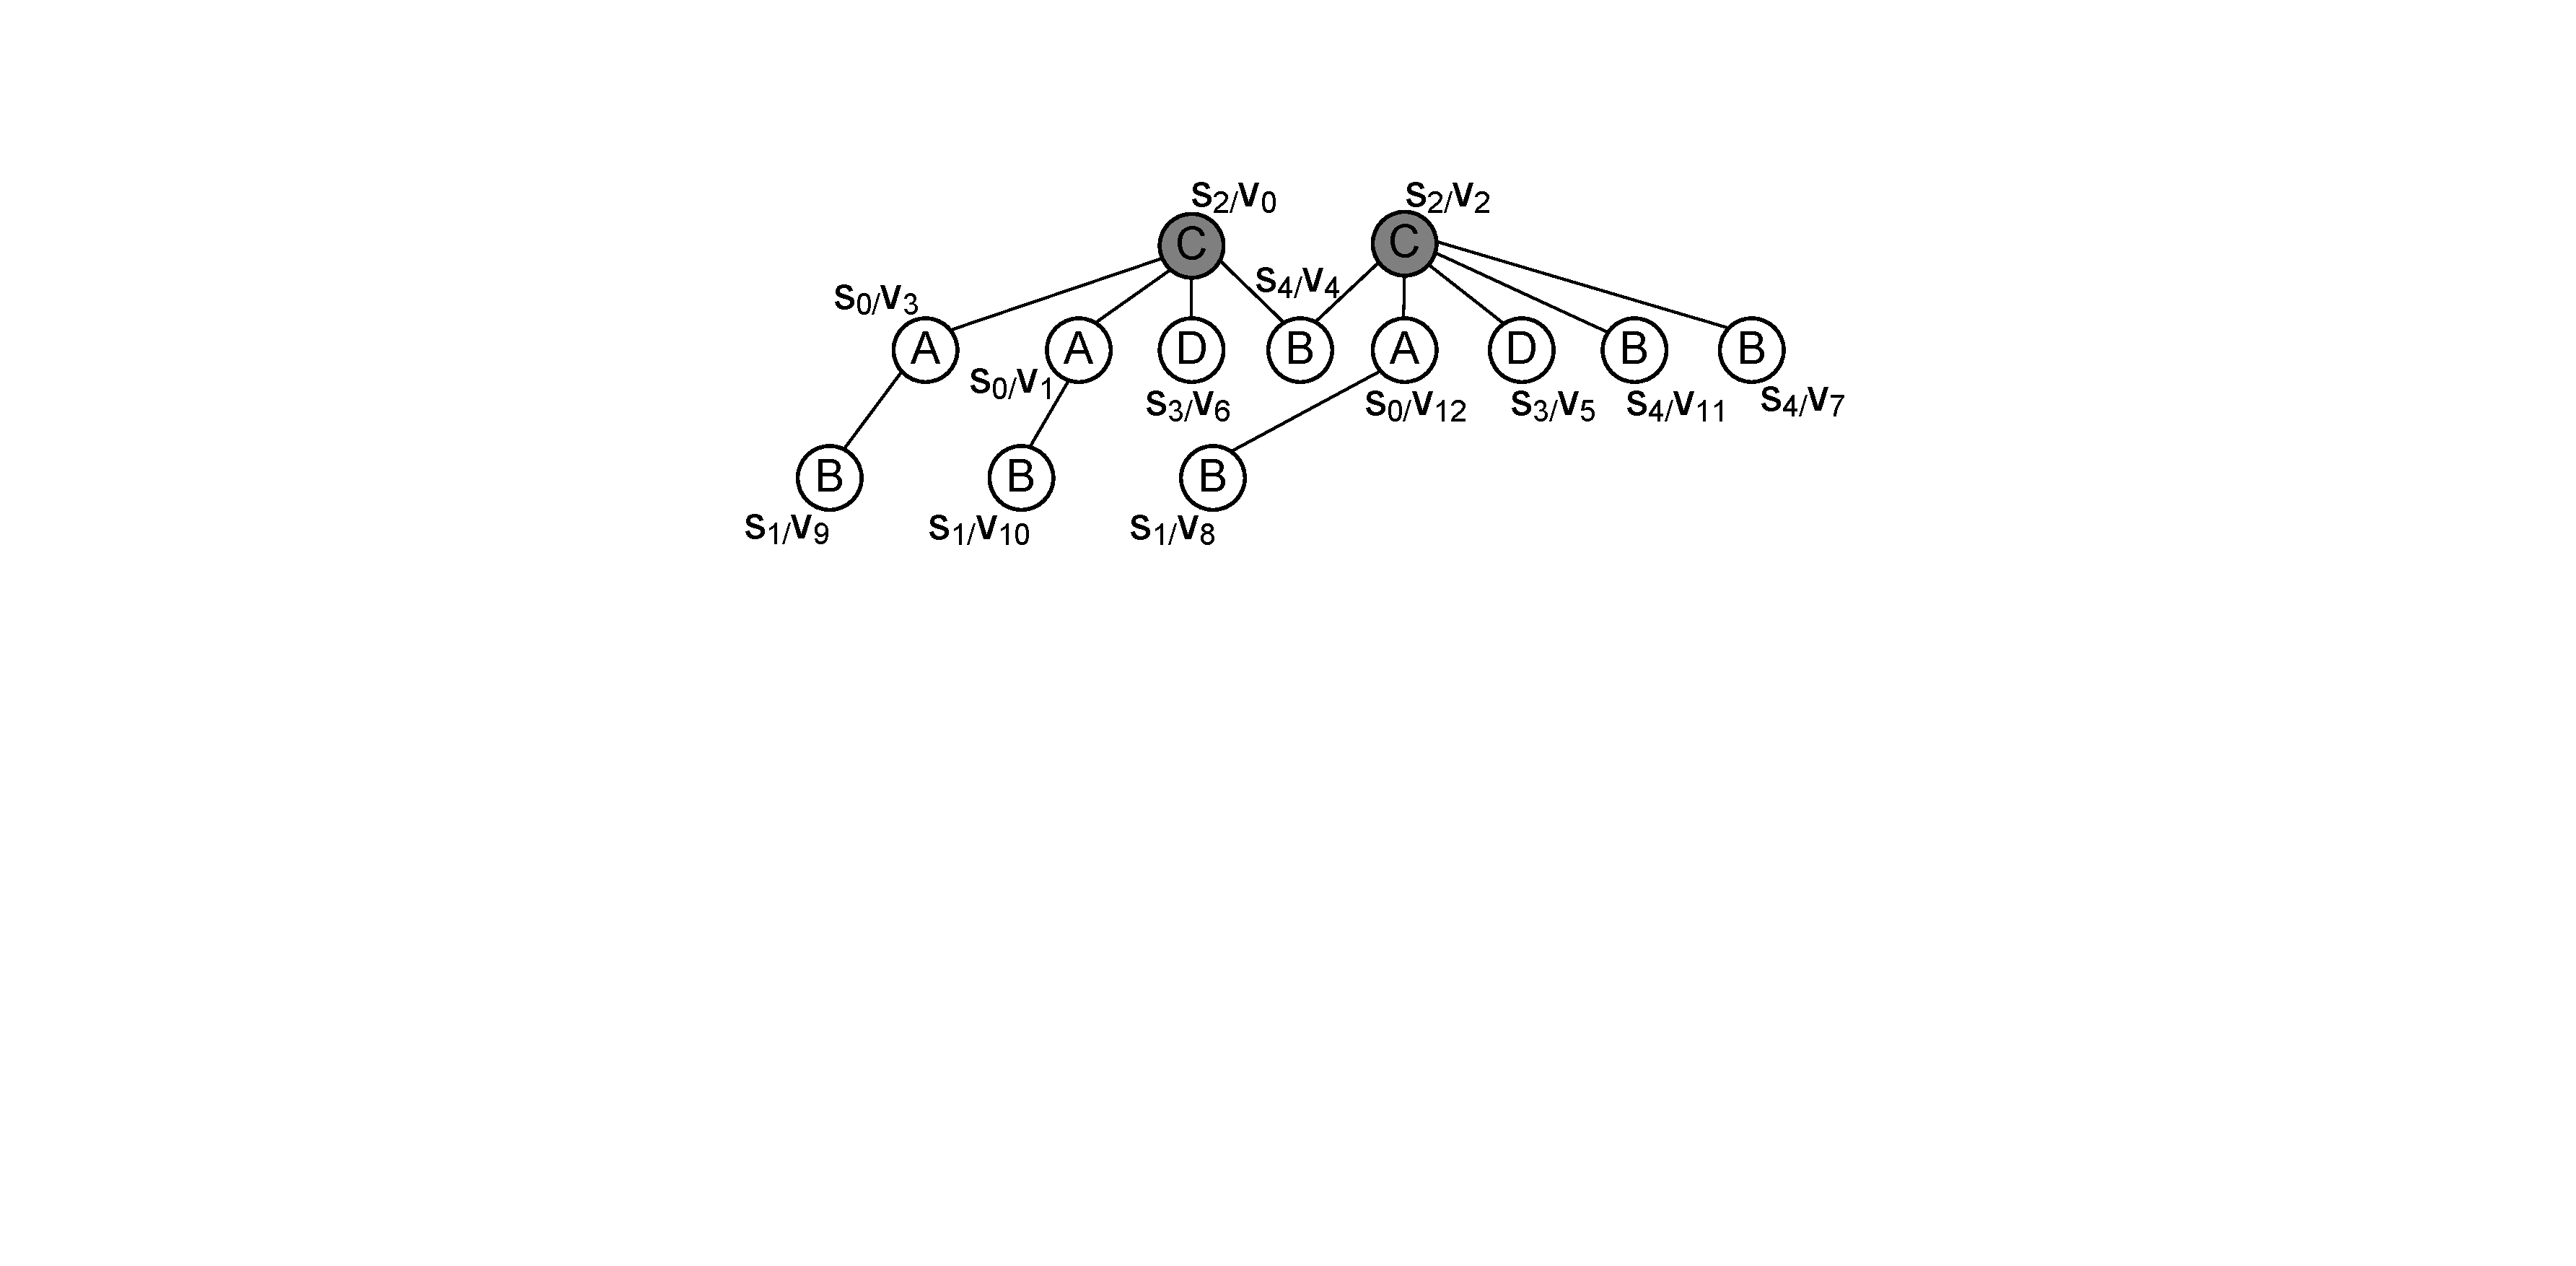
\includegraphics[scale=0.30]{images/tree_structure5}
\label{fig:tree_structure5}
}
\vspace{-2mm}
\caption{\scriptsize Figure \ref{fig:tree_structure0} is the subgraph pattern of $Q_1$, Figure \ref{fig:tree_structure2} is a replica of the occurrence of $Q_1$ in Figure \ref{fig:tree_structure1} without any backward edges (the dotted lines are the backward edges in $Q_1$). Figure \ref{fig:tree_structure4} is the same subgraph pattern $Q_2$ with Figure \ref{fig:tree_structure3}, with collection tree rooted at the group center $s_2$. Figure \ref{fig:tree_structure5} is the occurrence of $Q_2$ in data graph $G$.}
\label{fig:replica}
\vspace{-6mm}
\end{figure}
~\newline 
~\newline

%
Then, we consider the group center as the root of the tree. During the collection, the collection is initiated from the root of the tree.

% \subsubsection{Recursive Collection}\label{subsubsec:recursive}
% The collection could be completed by a naive straight forward traversal. However, we traverse by top-bottom manner and collect by bottom-top manner. This manner could help us to reduce duplicated calculation by saving the information of all ones subtrees.

\par Prior to the correlation computations for $Q$, we first update the distance index of proximity patterns using the data of proximity vertices. That is, for all $u\in Q$, for each $v\in Cor(u)$, $CorP(v)=CorP(v)\cup Q$.
\begin{lma}
\label{lemma:distance bidirection relation between vertices and patterns}
Let $Q$ be a subgraph, for all $v$ in data graph $G$, if $v\in \cup CorV(u),u\in Q$, then there must exists $Q\in CorP(v)$.
\end{lma}
\par After the update of the distance index, we operate the correlation calculation of subgraph $Q$. This process includes two phases.

\spara{$\bullet$ Collection Phase:} For each group center $c\in Center(Q)$, all instances of $Q$ including $c$ are enumerated in a depth-first manner similar to the recursive instances-enumeration technique of Algorithm 2. A set union of patterns contained in $CorP(u)$ is performed across every vertex $u$ of an instance group. At the same time, every vertex $v$ in the $proximity\ vertices\ map$ of $u$ ($CorV(u)$) records the proximity of pattern $Q$ in its $proximity\ patterns\ map$ ($CorP(v)$).

\begin{align}
Collect(c,Q)=\cup \{CorP(v)|v\in instance group\}
\end{align}
% Eventually, every group center has all the correlation corresponding to the collection tree.

\spara{$\bullet$ Computation Phase:} The correlation between patterns $Q_1$ and $Q_2$ is easily stated by calculating the count of instance groups of $Q_1$ that are positive instance group of $Q_2$.
\par Clearly, a instance group $I'_i$ of $Q_1$ is a positive instance group $Q_2$, i.e. $P(I'_i,Q_2,h)=1$ if and only if
\begin{align}
u=groupCenter(I'_i), Q_2\in Collect(u,Q_1)
\end{align}
Then, we sum all the results to get the correlation.
\begin{align}
\tau(Q_1,Q_2,h)=\sum_i^{\sigma(Q_1)} P(I'_i,Q_2,h)
\end{align}
Algorithm 4 summarises the steps described above.
\begin{algorithm}[h!]
\caption{Operate}\label{algo:operate}
\begin{algorithmic}[1] 
\REQUIRE data graph: $G$, hop value: $h$, initial distance index set: $Index$
\ENSURE 
\STATE $DFS\ List\leftarrow$ get rooted {\sf DFS} of $Q$ with $center$ as $root$
\FORALL{mappings $m$ of $center$ in $replica(Q)$}
\STATE $\mathbb{I}\leftarrow$ {set of all instances of $Q$ in $replica(Q)$ containing $m$ mapped to $center$}
\FORALL{vertex $u$ constituting an instance in $\mathbb{I}$}
\STATE $\forall v\in CorV(u)$, $CorP(v)\leftarrow CorP(v)\cup Q$
\STATE $Collect(m, Q)\leftarrow Collect(m, Q)\cup CorP(u)$
\ENDFOR
\ENDFOR
\FORALL{patterns $Q_k$ in set {\sf operated}}
\STATE $\tau(Q, Q_k, h)\leftarrow$ number of instance group centers $m$ s.t. $Q_k\in Collect(m, Q)$
\ENDFOR 
\STATE Update {\sf Top\ $k$} list with the computed correlation ($\tau$) values
\STATE {\sf operated} $\leftarrow$ {\sf operated} $\cup \ Q$
% \RETURN
\end{algorithmic}
\end{algorithm}
%append the "complete" collect-stat algorithm here 

% \begin{exple}
% 	In Figure \ref{fig:tree_structure5}, $v_0$ initiates a collection and it first goes to the deeper level until it reach the leaf, $v_9$, then it goes up from $v_9$ to $v_0$. Suppose $CorP(v_9)=\{Q_1\}$ and $CorP(v_3)=\{Q_2\}$, then $Collect(v_3,Q)=\{Q_1,Q_2\}$. This operation continues until $Collect(v_0,Q)$ is calculated. Moreover, since $Collect(v_4,Q)$ is calculated during the collection of $v_0$, it need not to be calculated again during the other collections. For example, in this case, $v_2$ initiates a collection and goes to $v_4$ and it can directly get the result of $Collect(v_4,Q)$ without going deeper.
% \end{exple}


\subsection{Avoiding Subgraph/Supergraph Correlation}\label{subsec:avoiding}
As we mentioned in Section \ref{sec:problem}, we do not want to consider the correlation of $Q_1,Q_2$ if $Q_1$ is a subgraph or a supergraph of $Q_2$. If $Q_2$ is extended from $Q_1$, we could easily know $Q_2$ is the supergraph of $Q_1$ and skip their correlation calculation. However, there are more troublesome conditions.


\begin{figure}[t!]
\centering
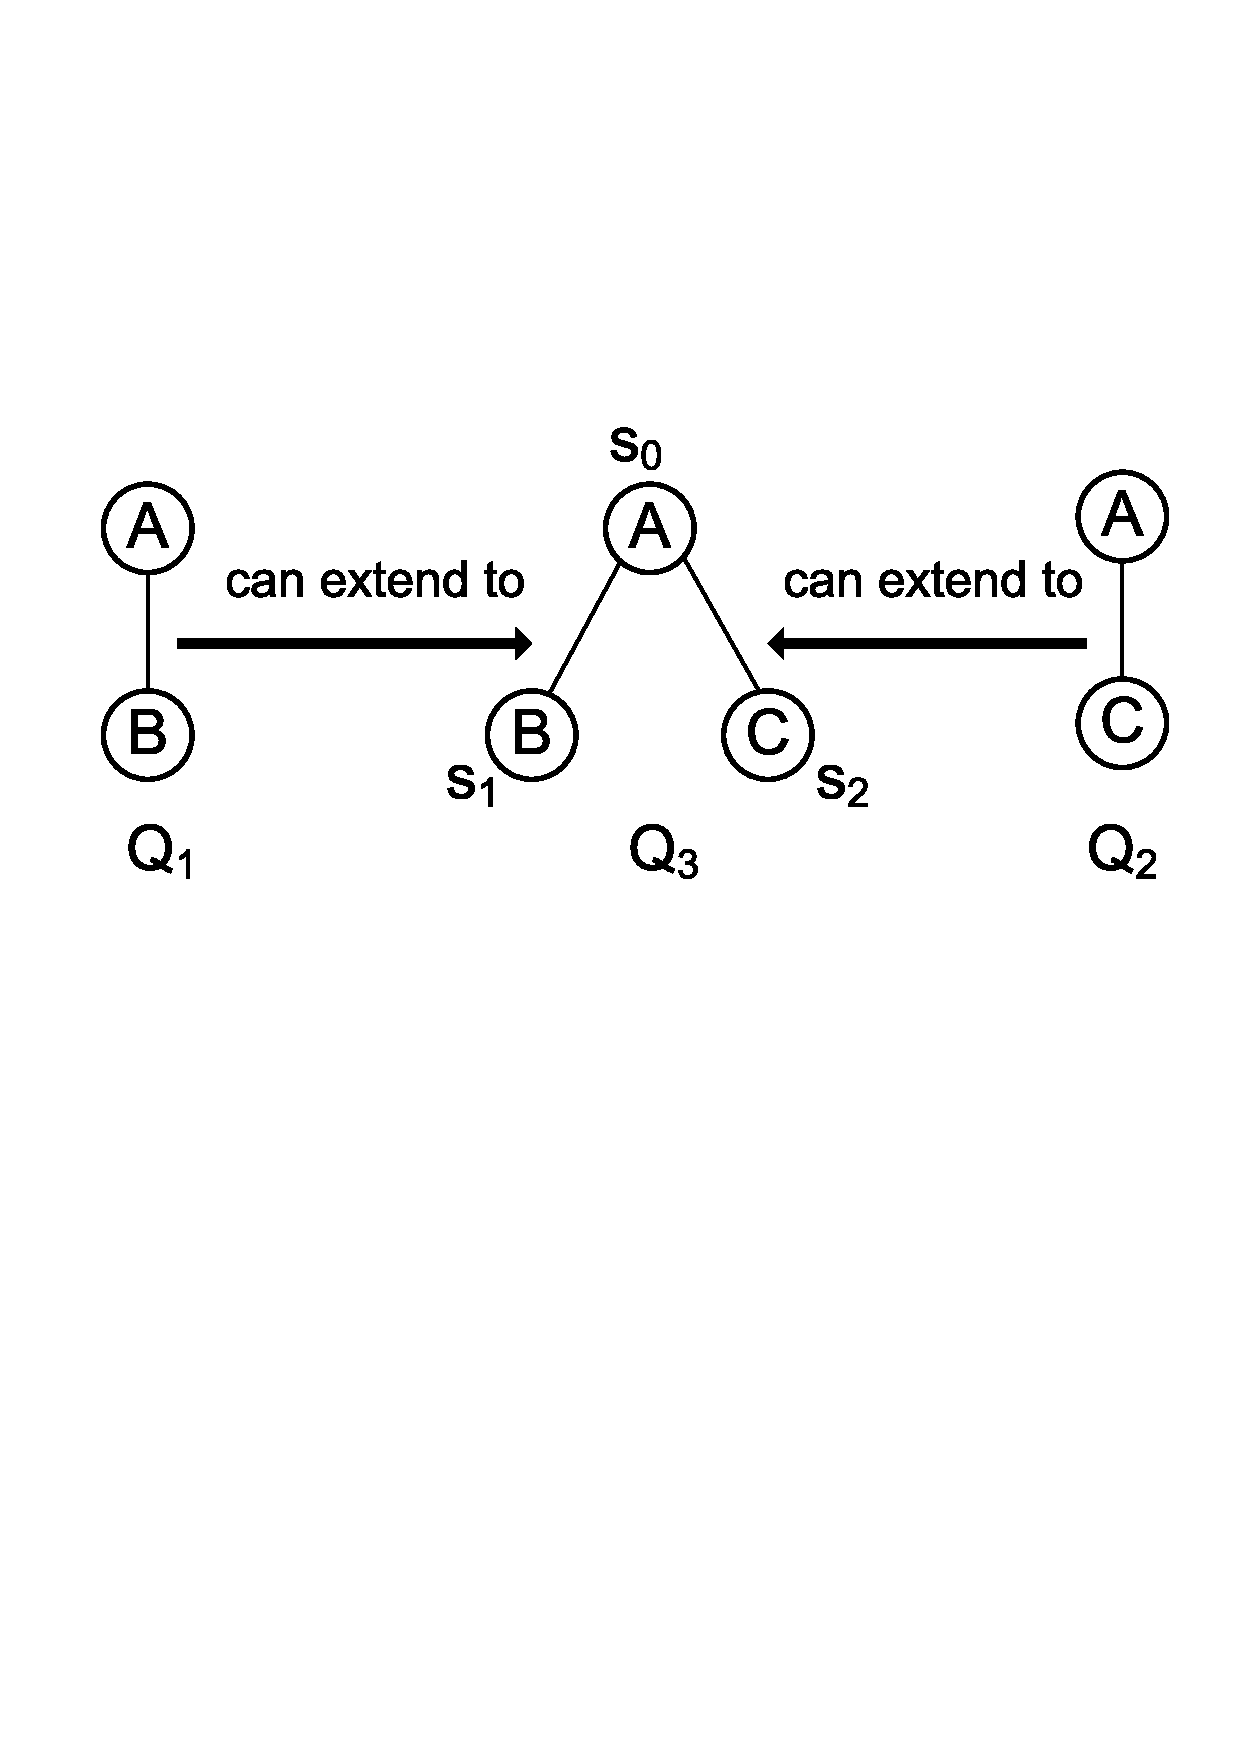
\includegraphics[scale=0.32]{images/avoiding}
\vspace{-2mm}
\caption{\scriptsize Subgraph $Q_1$ and $Q_2$ are the subgraphs of $Q_3$.}
\label{fig:avoiding}
\vspace{-6mm}
\end{figure}


\begin{exple}
	In Figure \ref{fig:avoiding}, suppose $Q_1$ extended to $Q_3$ and $Q_3$ knows that $Q_1$ is its subgraph. However, during {\sf Op($Q_3$)}, $Q_3$ must avoid the correlation $\tau(Q_3,Q_2,h)$ because $Q_2$ is also the subgraph of $Q_3$. 
\end{exple}


Obviously, we can not use subgraph isomorphism to check this relationship of $Q_1,Q_2$ before the correlation calculation since it is too expensive. We use following approach to rapidly get the answer.
\par We first add one more rule to best-first-search, if $\sigma(Q_1)=\sigma(Q_2)$, $Q_1$ has higher priority to be operated if and only if:
	\begin{align*} |V_{Q_1}|<|V_{Q_2}| \end{align*}
According to this rule, together with downward-closure, we could always guarantee that $Q_1$ is extended before $Q_2$.
\par For each subgraph $Q$, it maintain a subgraph set $SubRec(Q)$, recording all of its subgraphs. Under our assumption, $Q_1$ can extend to $Q_2$ so that $Q_2$ knows that $Q_1$ is the subgraph of $Q_2$ and all the subgraphs of $Q_1$ are also the subgraphs of $Q_2$. As a result, if $Q_1$ can extend to $Q_2$, then we operate $SubRec(Q_2)=SubRec(Q_2)\cap Q_1\cap SubRec(Q_1)$. As {\sf Op($Q$)} is occurring, if $Q_i\in SubRec(Q)$, we skip $\tau(Q,Q_i,h)$.
\newline
